\documentclass[12pt]{letter}

\usepackage{amsmath,amssymb}
\usepackage{nopageno}
\usepackage{enumitem}
\usepackage[a4paper, total={7.5in, 11.25in}]{geometry}
\usepackage{tikz}
\usepackage{pgfplots}
\pgfplotsset{compat=1.18}

\usetikzlibrary{calc,3d,decorations.pathmorphing,decorations.pathreplacing,decorations.markings,snakes,arrows.meta,patterns}
\tikzset{snake it/.style={decorate, decoration=snake}}

\begin{document}

Name: \hrulefill \quad Neptun code: \hrulefill

\begin{center}
(KTXFI1EBNF) Physics I. Test~2 Solutions \\
May~18,~2026 
\end{center}

\bigskip

\begin{enumerate}
\setcounter{enumi}{0}

\item Estimate the average depth of the Indian Ocean if a tsunami takes 24 hours to travel from Jakarta to Mogadishu. (Note: The propagation speed of shallow-water waves is $v=\sqrt{gh}$. The distance is $17000$\,km. $g=9.81\,\mathrm{m/s^{2}}.$)

%\bigskip

\begin{center}
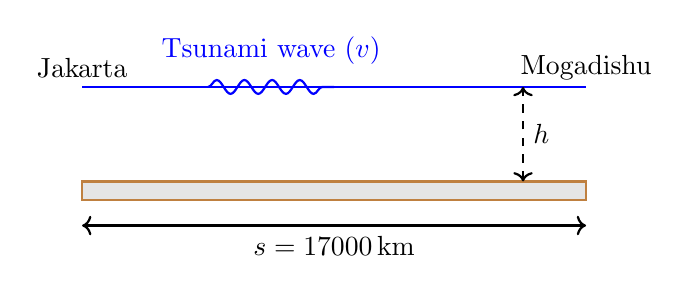
\begin{tikzpicture}[scale=0.8]
    % Ocean surface
    \draw[blue, thick] (0,1.5) -- (8,1.5);
    \draw[blue, thick, snake it] (2,1.5) -- (4,1.5);
    \node[blue, above] at (3,1.7) {Tsunami wave ($v$)};
    % Floor
    \draw[brown, thick, fill=gray!20] (0,0) rectangle (8,-0.3);
    % Depth arrow
    \draw[dashed, <->, thick] (7,0) -- (7,1.5) node[midway, right] {$h$};
    % Distance arrow
    \draw[<->, thick] (0,-0.7) -- (8,-0.7) node[midway, below] {$s = 17000\,\mathrm{km}$};
    \node at (0,1.8) {Jakarta};
    \node at (8,1.8) {Mogadishu};
\end{tikzpicture}
\end{center}

First, we convert the given time from hours to seconds:
$$t = 24\,\mathrm{hours} = 24 \cdot 3600\,\mathrm{s} = 86400\,\mathrm{s}$$
The distance $s$ in meters is:
$$s = 17000\,\mathrm{km} = 17 \cdot 10^6\,\mathrm{m}$$
The average propagation speed of the tsunami wave is:
$$v = \frac{s}{t} = \frac{17 \cdot 10^6\,\mathrm{m}}{86400\,\mathrm{s}} \approx 196.76\,\mathrm{m/s}$$
Using the formula for shallow-water waves:
$$v = \sqrt{gh} \implies v^2 = gh \implies h = \frac{v^2}{g}$$
Substituting the calculated velocity and $g = 9.81\,\mathrm{m/s^2}$:
$$h = \frac{(196.76\,\mathrm{m/s})^2}{9.81\,\mathrm{m/s^2}} \approx \frac{38714.50\,\mathrm{m^2/s^2}}{9.81\,\mathrm{m/s^2}} \approx 3946.43\,\mathrm{m}$$
The estimated average depth of the ocean along this path is approximately $3946.43\,\mathrm{m}$.

\hfill (10~points)

% ------------------------------------------------------------------------------------------------------------------------------------

\bigskip
\item A projectile is launched at an angle of $45^\circ$ with an initial velocity of $50\,\text{m/s}$ ($g=9.81\,\mathrm{m/s^{2}}$). 
Calculate:
\begin{enumerate}
    \item[(a)] The time to reach the peak of the trajectory.
    \item[(b)] The maximum height.
    \item[(c)] The horizontal range (impact distance).
    \item[(d)] The total time of flight.
\end{enumerate}     

%\bigskip

\begin{center}
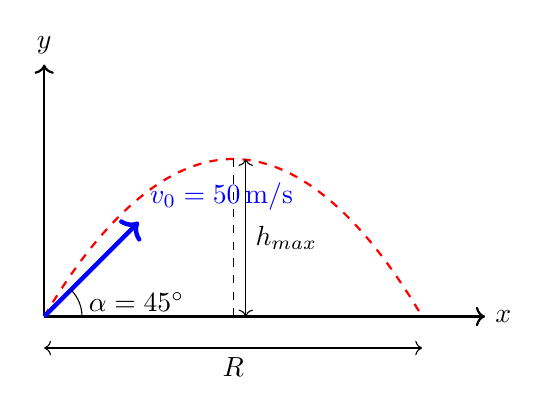
\begin{tikzpicture}[scale=0.8]
    \draw[->, thick] (0,0) -- (7,0) node[right] {$x$};
    \draw[->, thick] (0,0) -- (0,4) node[above] {$y$};
    % Trajectory
    \draw[dashed, red, thick] (0,0) parabola bend (3,2.5) (6,0);
    % Launch vector
    \draw[->, blue, ultra thick] (0,0) -- (1.5,1.5) node[above right] {$v_0=50\,\mathrm{m/s}$};
    \draw (0.6,0) arc (0:45:0.6) node[midway, right] {$\alpha=45^\circ$};
    % Max height
    \draw[dashed] (3,0) -- (3,2.5);
    \draw[<->] (3.2,0) -- (3.2,2.5) node[midway, right] {$h_{max}$};
    % Range
    \draw[<->] (0,-0.5) -- (6,-0.5) node[midway, below] {$R$};
\end{tikzpicture}
\end{center}

The initial components of the velocity are:
$$v_{0x} = v_0 \cos(45^\circ) = 50\,\mathrm{m/s} \cdot \frac{\sqrt{2}}{2} \approx 35.36\,\mathrm{m/s}$$
$$v_{0y} = v_0 \sin(45^\circ) = 50\,\mathrm{m/s} \cdot \frac{\sqrt{2}}{2} \approx 35.36\,\mathrm{m/s}$$
\begin{enumerate}
\item[(a)] At the peak of the trajectory, the vertical component of the velocity becomes zero ($v_y = 0\,\mathrm{m/s}$):
$$v_y = v_{0y} - gt_{peak} = 0 \implies t_{peak} = \frac{v_{0y}}{g} = \frac{35.36\,\mathrm{m/s}}{9.81\,\mathrm{m/s^2}} \approx 3.60\,\mathrm{s}$$

\item[(b)] The maximum height can be found using the vertical motion equation:
$$h_{max} = \frac{v_{0y}^2}{2g} = \frac{(35.36\,\mathrm{m/s})^2}{2 \cdot 9.81\,\mathrm{m/s^2}} \approx 63.71\,\mathrm{m}$$

\item[(c)] The horizontal range ($R$) is the horizontal distance traveled during the entire flight:
$$R = \frac{v_0^2 \sin(2\alpha)}{g} = \frac{(50\,\mathrm{m/s})^2 \sin(90^\circ)}{9.81\,\mathrm{m/s^2}} = \frac{2500\,\mathrm{m^2/s^2}}{9.81\,\mathrm{m/s^2}} \approx 254.84\,\mathrm{m}$$

\item[(d)] Since the launch and impact points are at the same horizontal level, the total time of flight is exactly twice the time to reach the peak:
$$t_{flight} = 2 \cdot t_{peak} = 2 \cdot 3.604\,\mathrm{s} \approx 7.21\,\mathrm{s}$$
\end{enumerate}

\hfill (10~points)

% ------------------------------------------------------------------------------------------------------------------------------------

\bigskip
\item We place a copper piece with a mass of 100 gramms and a temperature of $40{}^{\circ}C$ into 500 gramms of water at $80{}^{\circ}C$. What will be the common temperature? The specific heat capacity of copper is $3.85 \cdot 10^{2}\frac{J}{kg\,K}$ and the specific heat capacity of water is $4.19 \cdot 10^{3}\frac{J}{kg\,K}$.

\bigskip

\begin{center}
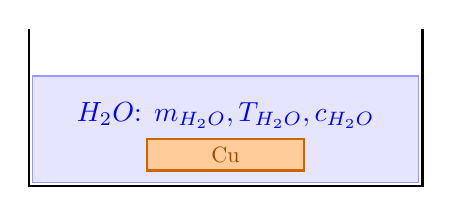
\begin{tikzpicture}
    % Beaker
    \draw[thick] (0,2) -- (0,0) -- (5,0) -- (5,2);
    % Water
    \draw[blue!40, fill=blue!10] (0.05,0.05) rectangle (4.95,1.4);
    \node[blue] at (2.5,0.9) {$H_{2}O$: $m_{H_{2}O}, T_{H_{2}O}, c_{H_{2}O}$};
    % Copper piece
    \draw[orange!80!black, fill=orange!40, thick] (1.5,0.2) rectangle (3.5,0.6);
    \node[orange!60!black, scale=0.8] at (2.5,0.4) {Cu};
\end{tikzpicture}
\end{center}

Let us use the principle of conservation of energy:
$$m_{Cu} c_{Cu} (T_f - T_{Cu}) + m_{H_{2}O} c_{H_{2}O} (T_f - T_{H_{2}O}) = 0$$
Given data converted to SI base units:
$$m_{Cu} = 100\,\mathrm{g} = 0.1\,\mathrm{kg}, \quad T_{Cu} = 40^\circ\mathrm{C}, \quad c_{Cu} = 385\,\mathrm{\frac{J}{kg \cdot K}}$$
$$m_{H_{2}O} = 500\,\mathrm{g} = 0.5\,\mathrm{kg}, \quad T_{H_{2}O} = 80^\circ\mathrm{C}, \quad c_{H_{2}O} = 4190\,\mathrm{\frac{J}{kg \cdot K}}$$

Solving for the final temperature $T_f$:
$$T_f = \frac{m_{Cu} c_{Cu} T_{Cu} + m_{H_{2}O} c_{H_{2}O} T_{H_{2}O}}{m_{Cu} c_{Cu} + m_{H_{2}O} c_{H_{2}O}} = \frac{0.1\,\mathrm{kg} \cdot 385\,\mathrm{\frac{J}{kg \cdot K}} \cdot 40^\circ\mathrm{C} + 0.5\,\mathrm{kg} \cdot 4190\,\mathrm{\frac{J}{kg \cdot K}} \cdot 80^\circ\mathrm{C}}{0.1\,\mathrm{kg} \cdot 385\,\mathrm{\frac{J}{kg \cdot K}} + 0.5\,\mathrm{kg} \cdot 4190\,\mathrm{\frac{J}{kg \cdot K}}}$$
$$T_f = \frac{1540\,\mathrm{\frac{J \cdot ^\circ C}{K}} + 167600\,\mathrm{\frac{J \cdot ^\circ C}{K}}}{38.5\,\mathrm{\frac{J}{K}} + 2095\,\mathrm{\frac{J}{K}}} = \frac{169140\,\mathrm{\frac{J \cdot ^\circ C}{K}}}{2133.5\,\mathrm{\frac{J}{K}}} \approx 79.28^\circ\mathrm{C}$$
The common equilibrium temperature will be approximately $79.28^\circ\mathrm{C}$.

\hfill (10~points)

% ------------------------------------------------------------------------------------------------------------------------------------

\bigskip
\item  What is the entropy change if the volume of $ m = 14\,\mathrm{g} $ of nitrogen changes from $ V_1 = 30\,\mathrm{l} \text{\ to\ } V_2 = 120\,\mathrm{l},$ and its temperature changes from $T_1 = 27^\circ\mathrm{C} \text{\ to\ } T_2 = 327^\circ\mathrm{C}?$ The molar mass is $ M = 28\,\mathrm{g/mol}$, $R=8.31\,\mathrm{\frac{J}{mol\cdot K}}$.

\bigskip

\begin{center}
\begin{tikzpicture}[scale=0.7]
    \draw[->, thick] (0,0) -- (5,0) node[right] {$V$};
    \draw[->, thick] (0,0) -- (0,4) node[above] {$T$};
    \draw[fill=blue!20] (1,1) circle (0.1) node[below left] {1};
    \draw[fill=red!20] (4,3) circle (0.1) node[above right] {2};
    \draw[dashed, ->, thick] (1,1) .. controls (2,2.5) .. (4,3) node[midway, above left] {$\Delta S$};
\end{tikzpicture}
\end{center}

Nitrogen ($\mathrm{N_2}$) is a diatomic ideal gas. The specific heat capacity at constant volume is $C_V = \frac{5}{2}R$, where $R = 8.314\,\mathrm{\frac{J}{mol \cdot K}}$.
First, calculate the number of moles ($n$):
$$n = \frac{m}{M} = \frac{14\,\mathrm{g}}{28\,\mathrm{g/mol}} = 0.5\,\mathrm{mol}$$
Convert temperatures to Kelvin:
$$T_1 = 27\,\mathrm{{}^{\circ}C} + 273.15\,\mathrm{K} = 300.15\,\mathrm{K}$$
$$T_2 = 327\,\mathrm{{}^{\circ}C} + 273.15\,\mathrm{K} = 600.15\,\mathrm{K}$$
The total entropy change ($\Delta S$) is given by:
$$\Delta S = n \left(\frac{5}{2}R\right) \ln\left(\frac{T_2}{T_1}\right) + n R \ln\left(\frac{V_2}{V_1}\right)$$
Substitute the corresponding values:
$$\Delta S = 0.5\,\mathrm{mol} \cdot \left(2.5 \cdot 8.314\,\mathrm{\frac{J}{mol \cdot K}}\right) \ln\left(\frac{600.15\,\mathrm{K}}{300.15\,\mathrm{K}}\right) + 0.5\,\mathrm{mol} \cdot 8.314\,\mathrm{\frac{J}{mol \cdot K}} \ln\left(\frac{0.120\,\mathrm{m^{3}}}{0.030\,\mathrm{m^3}}\right)$$
$$\Delta S = 10.3925\,\mathrm{\frac{J}{K}} \cdot \ln(2) + 4.157\,\mathrm{\frac{J}{K}} \cdot \ln(4) \approx 7.204\,\mathrm{\frac{J}{K}} + 5.763\,\mathrm{\frac{J}{K}} = 12.97\,\mathrm{\frac{J}{K}}$$
The entropy change of the nitrogen gas is approximately $12.97\,\mathrm{\frac{J}{K}}$.

\hfill (10~points)

% ------------------------------------------------------------------------------------------------------------------------------------

\bigskip
\item Determine the acceleration of a proton ($m = 1.67 \cdot 10^{-27}\,\mathrm{kg}$, $e=1.6\cdot 10^{-19}\,\mathrm{C}$) in an electric field of strength $ E = 10000\,\mathrm{N/C}. $ How many times greater is this acceleration than the acceleration due to gravity?

%\bigskip

\begin{center}
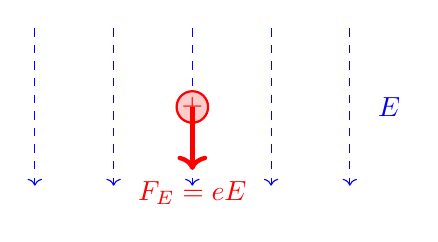
\begin{tikzpicture}
    % Electric Field lines
    \foreach \x in {0,1,2,3,4}
        \draw[blue, ->, dashed] (\x,2) -- (\x,0);
    \node[blue] at (4.5, 1) {$E$};
    % Proton
    \draw[red, fill=red!20, thick] (2,1) circle (0.2) node {$+$};
    \draw[->, ultra thick, red] (2,1) -- (2,0.2) node[below] {$F_E = eE$};
\end{tikzpicture}
\end{center}

The electrostatic force acting on the proton is:
$$F_E = e \cdot E$$
According to Newton's second law, the acceleration $a$ is:
$$a = \frac{e \cdot E}{m}$$
Substituting the given constants:
$$a = \frac{1.6 \cdot 10^{-19}\,\mathrm{C} \cdot 10000\,\mathrm{N/C}}{1.67 \cdot 10^{-27}\,\mathrm{kg}} \approx 9.58 \cdot 10^{11}\,\mathrm{m/s^2}$$

To find how many times greater this is than gravity ($g = 9.81\,\mathrm{m/s^2}$):
$$\text{Ratio} = \frac{a}{g} = \frac{9.581 \cdot 10^{11}\,\mathrm{m/s^2}}{9.81\,\mathrm{m/s^2}} \approx 9.77 \cdot 10^{10}$$
The acceleration of the proton is approximately $9.58 \cdot 10^{11}\,\mathrm{m/s^2}$, which is roughly $9.77 \cdot 10^{10}$ times greater than gravity.

\hfill (10~points)

\end{enumerate}

% ------------------------------------------------------------------------------------------------------------------------------------

Requirement for obtaining the course signature: achieving at least 40\% (20\,points) on the midterm exam.

Grades: 0--25 points: Fail (1), 26--30 points: Pass (2), 31--37 points: Satisfactory (3), 38--45 points:~Good~(4), 46--50 points: Excellent (5).

\rightline{Dr.~Gabor FACSKO}
\rightline{\textit{facsko.gabor@uni-obuda.hu}}

\vfill

\end{document}
